\hypertarget{barcode_8inc}{
\section{include/barcode.inc File Reference}
\label{barcode_8inc}\index{include/barcode.inc@{include/barcode.inc}}
}
Functions for the handling of different barcodes. 

\subsection*{Functions}
\begin{CompactItemize}
\item 
\hyperlink{barcode_8inc_6d3645af0ef526e4f64d28dcbdceb74f}{checkBarcode} (\$barcode)
\item 
\hyperlink{barcode_8inc_e10c37e4f9f9b7c6617a388351a27c99}{getBarcodeInfo} (\$barcode)
\end{CompactItemize}


\subsection{Detailed Description}
Functions for the handling of different barcodes. 

This file currently deals with the handling of barcodes and getting the information associated with them. 

Definition in file \hyperlink{barcode_8inc-source}{barcode.inc}.

\subsection{Function Documentation}
\hypertarget{barcode_8inc_6d3645af0ef526e4f64d28dcbdceb74f}{
\index{barcode.inc@{barcode.inc}!checkBarcode@{checkBarcode}}
\index{checkBarcode@{checkBarcode}!barcode.inc@{barcode.inc}}
\subsubsection{\setlength{\rightskip}{0pt plus 5cm}checkBarcode (\$ {\em barcode})}}
\label{barcode_8inc_6d3645af0ef526e4f64d28dcbdceb74f}


Checks to see if a valid, handalable, barcode was entered. \begin{Desc}
\item[Parameters:]
\begin{description}
\item[{\em \$barcode}]The Barcode to be checked \end{description}
\end{Desc}
\begin{Desc}
\item[Returns:]The type of barcode entered if valid, FALSE if it is not \end{Desc}


Array containinf info on the given UPC 

Definition at line 16 of file barcode.inc.

References XMLRPC\_\-prepare(), and XMLRPC\_\-request().

\begin{Code}\begin{verbatim}16                                 {
20   $result = XMLRPC_request('dev.upcdatabase.com', '/rpc', 'lookupUPC', array(XMLRPC_prepare($barcode)));
21   if ($result[1] != 'Error: Invalid length') {
22     if (strlen($barcode) == 12) {
23       return 'upca';
24     }
25     else if (strlen($barcode) == 13) {
26       return 'ean13';
27     }
28     else {
29       return FALSE;
30     }
31   }
32   else {
33     return FALSE;
34   }
35 }
\end{verbatim}
\end{Code}




Here is the call graph for this function:\nopagebreak
\begin{figure}[H]
\begin{center}
\leavevmode
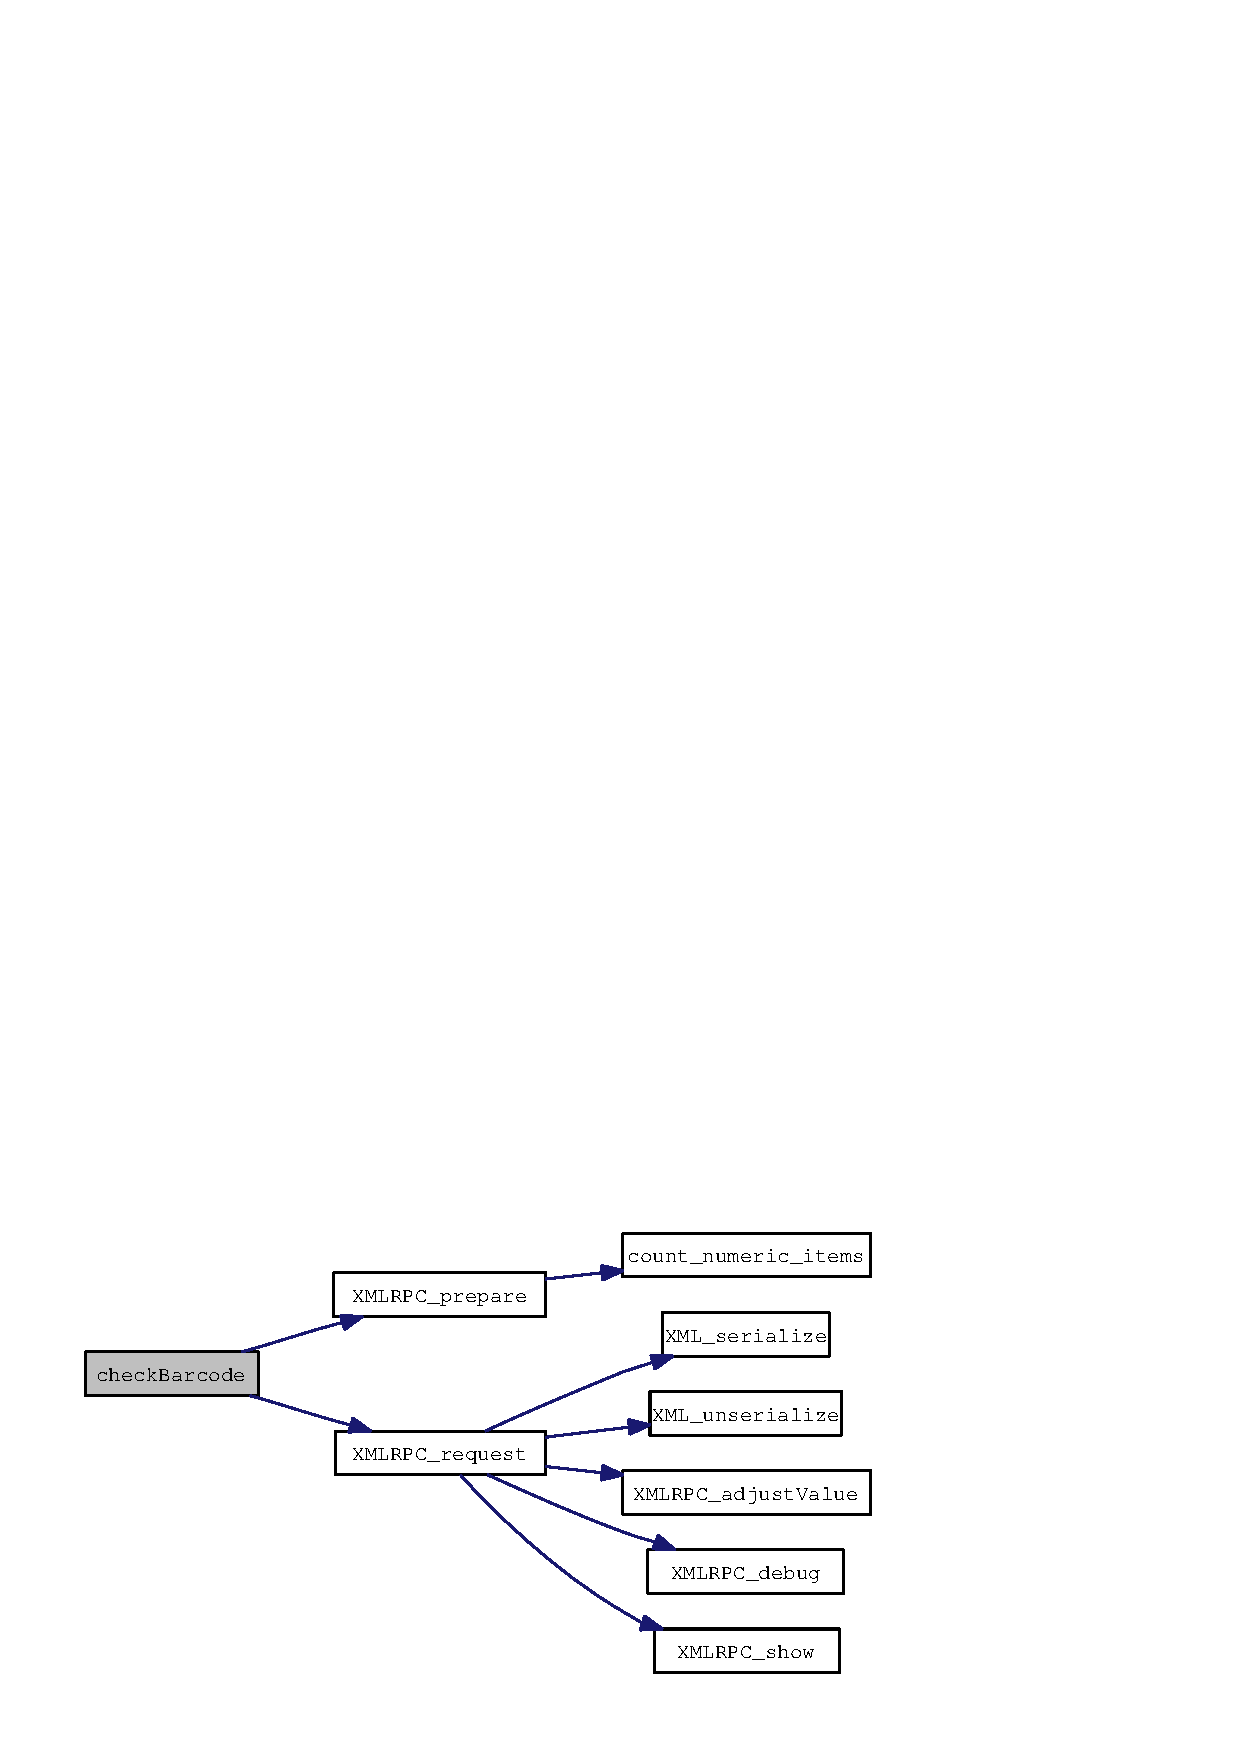
\includegraphics[width=211pt]{barcode_8inc_6d3645af0ef526e4f64d28dcbdceb74f_cgraph}
\end{center}
\end{figure}
\hypertarget{barcode_8inc_e10c37e4f9f9b7c6617a388351a27c99}{
\index{barcode.inc@{barcode.inc}!getBarcodeInfo@{getBarcodeInfo}}
\index{getBarcodeInfo@{getBarcodeInfo}!barcode.inc@{barcode.inc}}
\subsubsection{\setlength{\rightskip}{0pt plus 5cm}getBarcodeInfo (\$ {\em barcode})}}
\label{barcode_8inc_e10c37e4f9f9b7c6617a388351a27c99}


Output Barcode Info \begin{Desc}
\item[Parameters:]
\begin{description}
\item[{\em \$barcode}]The barcode to lookup \end{description}
\end{Desc}
\begin{Desc}
\item[Returns:]HTML code to create the info area \end{Desc}
\begin{Desc}
\item[See also:]\hyperlink{barcode_8inc_6d3645af0ef526e4f64d28dcbdceb74f}{checkBarcode} \end{Desc}


Hold the HTML code to be outputted

Array containinf info on the given UPC 

Definition at line 43 of file barcode.inc.

References getImages(), XMLRPC\_\-prepare(), and XMLRPC\_\-request().

\begin{Code}\begin{verbatim}43                                   {
47   $output = '';
48   $output .= '<div id="upc">';
49   $output .= '<img src="upcimg.php?upc=' . $barcode . '" />';
50   $output .= '</div>';
51 
55   $result = XMLRPC_request('dev.upcdatabase.com', '/rpc', 'lookupUPC', array(XMLRPC_prepare($barcode)));
56   /*if ($debug) */var_dump($result);
57   echo getImages($result[1]['description']);
58   if ($result[1]['found']) {
59     extract($result[1], EXTR_PREFIX_ALL, 'barcode');
60     $output .= <<<_HTML
61     <div id="info">
62       <table align="center">
63         <tr>
64           <td class="title">Country</td>
65           <td>$barcode_issuerCountry</td>
66         </tr>
67         <tr>
68           <td class="title">Description</td>
69           <td>$barcode_description</td>
70         </tr>
71         <tr>
72           <td class="title">Size</td>
73           <td>$barcode_size</td>
74         </tr>
75       </table>
76       <a href="http://www.upcdatabase.com/editform.asp?upc=$barcode">Modify this entry</a>
77       <a href="http://www.upcdatabase.com/deleteform.asp?upc=$barcode">Delete this entry</a>
78     </div>
79 _HTML;
80   }
81   else {
82     $output .= 'Product Not Found!<br />';
83     $output .= '<a href="http://www.upcdatabase.com/addform.asp?upc=' . $barcode . '">Add this item to the database</a>';
84   }
85 
86   return $output;
87 }\end{verbatim}
\end{Code}




Here is the call graph for this function:\nopagebreak
\begin{figure}[H]
\begin{center}
\leavevmode
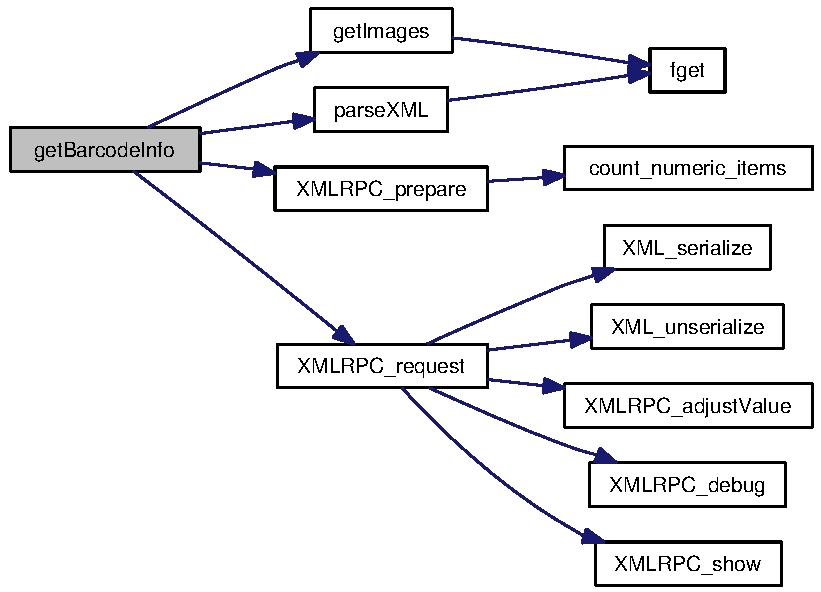
\includegraphics[width=215pt]{barcode_8inc_e10c37e4f9f9b7c6617a388351a27c99_cgraph}
\end{center}
\end{figure}
